\section{Question 4}

\subsection{How can endogenous fertility adjustments affect the impact of a child subsidy reform?}

\paragraph{Income effect on fertility.}

A child subsidy increases household resources when children are present, effectively lowering the net cost of having a child. This raises the lifetime resources associated with fertility and can make children more affordable. As a result, households may choose to have more children, provided the subsidy offsets part of the additional disutility of work associated with children captured by $\beta_1$.

\paragraph{Substitution effect on fertility.}

A subsidy also changes relative prices. When the monetary cost of children falls, the relative ``price'' of having children decreases compared to market consumption and labour income. Households may therefore substitute away from labour supply and toward childrearing.

\paragraph{Implications for policy evaluation.}

In the baseline model, policy changes only affect labour supply conditional on having a child. If fertility were endogenous, a subsidy could increase the number of births, as couples would enter states with children and where labour supply would be more costly. This is just not always true, as the increase in children has been shown to only be big short term, but very little long term, by \cite{Adda2017}.

\begin{figure}[H]
    \centering
    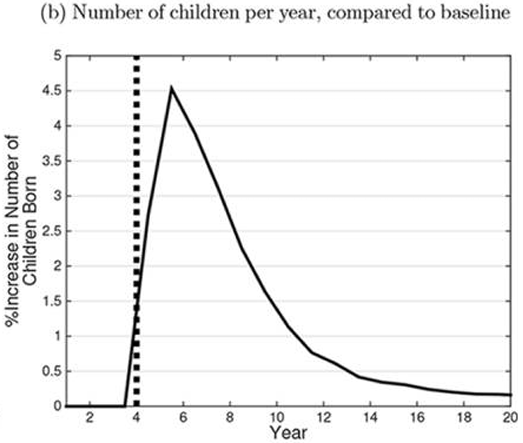
\includegraphics[width=0.5\linewidth]{Billeder/Adda.png}
    \caption{The short term effect of introducing a child premium.}
    \label{fig:placeholder}
\end{figure}